\documentclass[aspectratio=169,10pt]{beamer}
\usetheme{metropolis}
\metroset{block=fill}
\usepackage{appendixnumberbeamer}
\usepackage{booktabs}
\usepackage{xeCJK}
\usepackage{graphicx}
\usepackage{tikz}
\usetikzlibrary{shapes,arrows,positioning,fit,backgrounds}
\usepackage{amsmath}
\usepackage{fontawesome5}
\usepackage{pifont}
\usepackage{hyperref}

% Color definitions
\definecolor{primaryblue}{RGB}{0,83,155}
\definecolor{accentorange}{RGB}{230,126,34}
\definecolor{successgreen}{RGB}{39,174,96}
\definecolor{lightgray}{RGB}{236,240,241}

\setbeamercolor{frametitle}{bg=primaryblue}
\setbeamercolor{progress bar}{fg=accentorange}

% Check/cross marks for tables
\newcommand{\cmark}{\textcolor{successgreen}{\ding{51}}}
\newcommand{\xmark}{\textcolor{red}{\ding{55}}}

\title{AI, Software Engineering, and Compilers}
\subtitle{A Survey of AI-Native Software Development}
\author{Paper Reading \& Summary}
\date{2026}
\institute{PhD Seminar}

\begin{document}

\maketitle

%=============================================================================
\section{Introduction}
%=============================================================================

\begin{frame}{Outline}
    \tableofcontents
\end{frame}

\begin{frame}{The Changing Landscape of Software Engineering}
    \begin{columns}
    \column{0.5\textwidth}
    \textbf{Traditional Software Engineering}
    \begin{itemize}
        \item Human writes code
        \item Compiler translates to machine code
        \item Static, deterministic process
        \item Focus on correctness \& performance
    \end{itemize}
    
    \column{0.5\textwidth}
    \textbf{AI-Native Software Engineering}
    \begin{itemize}
        \item Human expresses \alert{intent}
        \item AI generates/transforms code
        \item Dynamic, probabilistic process
        \item Focus on correctness + cost + latency
    \end{itemize}
    \end{columns}
    
    \vspace{1em}
    \begin{block}{Key Insight}
    LLMs can now understand, generate, and transform code — blurring the line between human intent and executable software.
    \end{block}
\end{frame}

\begin{frame}{Papers We Cover Today}
    \begin{enumerate}
        \item \textbf{Challenges and Paths Towards AI for Software Engineering} \\
        {\small Gu et al., 2025 — Task taxonomy \& challenges}
        
        \item \textbf{AI Agentic Programming: A Survey} \\
        {\small Wang et al., 2025 — Coding agents taxonomy \& architectures}
        
        \item \textbf{The New Compiler Stack} \\
        {\small Zhang et al., 2026 — LLM + Compiler synergy survey (159 papers)}
        
        \item \textbf{Compiler.next: Search-Based Compiler for SE 3.0} \\
        {\small Cogo et al., 2025 — Intent-to-software compilation}
    \end{enumerate}
\end{frame}

%=============================================================================
\section{AI for Software Engineering: Tasks}
%=============================================================================

\begin{frame}{Task Taxonomy in AI for SE}
    \begin{columns}[T]
    \column{0.5\textwidth}
    \textbf{Code Generation}
    \begin{itemize}
        \item Code completion (tab completion)
        \item Natural language → code
        \item Full program synthesis
    \end{itemize}
    
    \textbf{Code Transformation}
    \begin{itemize}
        \item Refactoring
        \item Migration \& Translation
        \item Optimization
    \end{itemize}
    
    \column{0.5\textwidth}
    \textbf{Testing \& Analysis}
    \begin{itemize}
        \item Unit test generation
        \item Fuzzing
        \item Bug detection \& repair
    \end{itemize}
    
    \textbf{Maintenance}
    \begin{itemize}
        \item Documentation
        \item Code review
        \item Question answering
    \end{itemize}
    \end{columns}
    
    \vspace{0.5em}
    \begin{alertblock}{Beyond Code Generation}
    Most research focuses on code generation, but real SE involves many other tasks!
    \end{alertblock}
\end{frame}

\begin{frame}{Three Measures for Categorizing Tasks}
    \begin{columns}[T]
    \column{0.33\textwidth}
    \textbf{\faRuler~Scope}
    \begin{itemize}
        \item Function-level
        \item File/Class-level
        \item Project-level
    \end{itemize}
    {\small Examples: HumanEval (function) vs SWE-Bench (project)}
    
    \column{0.33\textwidth}
    \textbf{\faBrain~Logical Complexity}
    \begin{itemize}
        \item Low: CRUD apps
        \item Medium: LeetCode
        \item High: Competition, crypto
    \end{itemize}
    
    \column{0.33\textwidth}
    \textbf{\faUsers~Human Intervention}
    \begin{itemize}
        \item Low: AI as tool
        \item Medium: Collaborator
        \item High: AI as agent
    \end{itemize}
    \end{columns}
    
    \vspace{1em}
    \begin{exampleblock}{Goal}
    AI should be capable across all three dimensions — not just simple, isolated code completion.
    \end{exampleblock}
\end{frame}

%=============================================================================
\section{AI Coding Agents}
%=============================================================================

\begin{frame}{What is AI Agentic Programming?}
    \begin{block}{Definition}
    LLM-based agents that \textbf{autonomously plan, execute, and refine} software development tasks through iterative, tool-augmented workflows.
    \end{block}
    
    \vspace{0.5em}
    \textbf{Key Properties:}
    \begin{itemize}
        \item \textbf{Autonomy}: Make decisions without continuous human supervision
        \item \textbf{Interactivity}: Engage with external tools (compilers, debuggers, etc.)
        \item \textbf{Iterative Refinement}: Improve outputs based on feedback
        \item \textbf{Goal-Oriented}: Pursue high-level objectives, not just respond to prompts
    \end{itemize}
    
    \vspace{0.5em}
    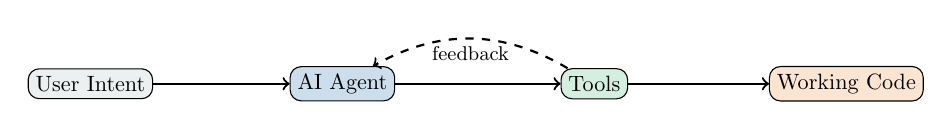
\begin{tikzpicture}[scale=0.8, every node/.style={scale=0.8}]
        \node[draw, rounded corners, fill=lightgray] (user) at (0,0) {User Intent};
        \node[draw, rounded corners, fill=primaryblue!20] (agent) at (4,0) {AI Agent};
        \node[draw, rounded corners, fill=successgreen!20] (tools) at (8,0) {Tools};
        \node[draw, rounded corners, fill=accentorange!20] (code) at (12,0) {Working Code};
        
        \draw[->, thick] (user) -- (agent);
        \draw[->, thick] (agent) -- (tools);
        \draw[->, thick] (tools) -- (code);
        \draw[->, thick, dashed] (tools) to[bend right=30] node[below]{\small feedback} (agent);
    \end{tikzpicture}
\end{frame}

\begin{frame}{Agent Behavior Dimensions}
    \begin{columns}[T]
    \column{0.5\textwidth}
    \textbf{1. Reactivity vs Proactivity}
    \begin{itemize}
        \item \textcolor{gray}{Reactive}: Respond to prompts (Copilot)
        \item \textcolor{successgreen}{Proactive}: Initiate sub-tasks, plan ahead
    \end{itemize}
    
    \vspace{0.5em}
    \textbf{2. Single-turn vs Multi-turn}
    \begin{itemize}
        \item \textcolor{gray}{Single-turn}: No context memory
        \item \textcolor{successgreen}{Multi-turn}: Maintain state across interactions
    \end{itemize}
    
    \column{0.5\textwidth}
    \textbf{3. Tool-Augmented vs Standalone}
    \begin{itemize}
        \item \textcolor{gray}{Standalone}: LLM reasoning only
        \item \textcolor{successgreen}{Tool-augmented}: Compilers, debuggers, etc.
    \end{itemize}
    
    \vspace{0.5em}
    \textbf{4. Static vs Adaptive}
    \begin{itemize}
        \item \textcolor{gray}{Static}: Fixed workflows
        \item \textcolor{successgreen}{Adaptive}: Modify strategies based on feedback
    \end{itemize}
    \end{columns}
\end{frame}

\begin{frame}{Agent Evolution: From Reactive to Autonomous}
    \begin{center}
    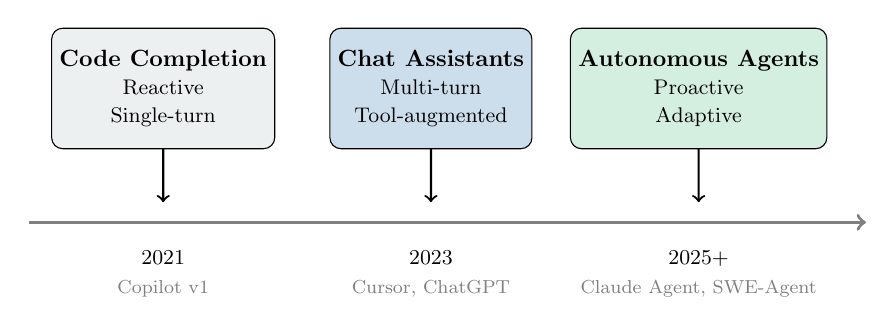
\begin{tikzpicture}[scale=0.85, every node/.style={scale=0.85}]
        % Timeline arrow
        \draw[->, very thick, gray] (-0.5,0) -- (12,0);
        
        % Stage 1
        \node[draw, rounded corners, fill=lightgray, minimum width=2.8cm, minimum height=1.8cm, align=center] (s1) at (1.5,2) {\textbf{Code Completion}\\{\small Reactive}\\{\small Single-turn}};
        \draw[->, thick] (s1) -- (1.5,0.3);
        \node[below] at (1.5,-0.3) {\small 2021};
        
        % Stage 2
        \node[draw, rounded corners, fill=primaryblue!20, minimum width=2.8cm, minimum height=1.8cm, align=center] (s2) at (5.5,2) {\textbf{Chat Assistants}\\{\small Multi-turn}\\{\small Tool-augmented}};
        \draw[->, thick] (s2) -- (5.5,0.3);
        \node[below] at (5.5,-0.3) {\small 2023};
        
        % Stage 3
        \node[draw, rounded corners, fill=successgreen!20, minimum width=2.8cm, minimum height=1.8cm, align=center] (s3) at (9.5,2) {\textbf{Autonomous Agents}\\{\small Proactive}\\{\small Adaptive}};
        \draw[->, thick] (s3) -- (9.5,0.3);
        \node[below] at (9.5,-0.3) {\small 2025+};
        
        % Examples
        \node[font=\footnotesize, gray] at (1.5,-1) {Copilot v1};
        \node[font=\footnotesize, gray] at (5.5,-1) {Cursor, ChatGPT};
        \node[font=\footnotesize, gray] at (9.5,-1) {Claude Agent, SWE-Agent};
    \end{tikzpicture}
    \end{center}
    
    \vspace{0.5em}
    \begin{block}{Key Capabilities of Modern Agents}
    \begin{itemize}
        \item \textbf{Proactive}: Decompose tasks, plan ahead, initiate sub-tasks
        \item \textbf{Multi-turn}: Maintain context across interactions
        \item \textbf{Tool-augmented}: Integrate compilers, debuggers, test frameworks
        \item \textbf{Adaptive}: Learn from feedback, revise strategies
    \end{itemize}
    \end{block}
\end{frame}

%=============================================================================
\section{LLMs in Compilers}
%=============================================================================

\begin{frame}{The New Compiler Stack: LLM Integration}
    \textbf{How are LLMs integrated into compilation?}
    
    \vspace{1em}
    \begin{columns}[T]
    \column{0.33\textwidth}
    \textbf{\faMousePointer~Selector}
    \begin{itemize}
        \item Choose from predefined options
        \item e.g., compiler flags, pass ordering
        \item Safe: only valid choices
        \item Limited creative potential
    \end{itemize}
    
    \column{0.33\textwidth}
    \textbf{\faExchange*~Translator}
    \begin{itemize}
        \item Direct code transformation
        \item Transpilation, optimization
        \item High potential
        \item Verification challenge
    \end{itemize}
    
    \column{0.33\textwidth}
    \textbf{\faCode~Generator}
    \begin{itemize}
        \item Generate compiler code itself
        \item Meta-level approach
        \item Generates transformation scripts
        \item Most complex
    \end{itemize}
    \end{columns}
\end{frame}

\begin{frame}{LLM-Compiler Applications: Success Stories}
    \begin{columns}[T]
    \column{0.5\textwidth}
    \textbf{\faRocket~Code Transpilation}
    \begin{itemize}
        \item C → Rust (memory safety)
        \item CUDA → HIP (portability)
        \item Legacy COBOL → Modern langs
    \end{itemize}
    
    \vspace{0.3em}
    \textbf{\faMemory~IR Optimization}
    \begin{itemize}
        \item \textbf{LLMCompiler}: Pre-trained on LLVM IR
        \item Flag/pass selection (replacing heuristics)
        \item Code size reduction
    \end{itemize}
    
    \column{0.5\textwidth}
    \textbf{\faMicrochip~Hardware Synthesis}
    \begin{itemize}
        \item Natural language → Verilog/VHDL
        \item High-level synthesis optimization
    \end{itemize}
    
    \vspace{0.3em}
    \textbf{\faBug~Automated Repair}
    \begin{itemize}
        \item Bug fix as translation task
        \item Compiler error → fix suggestion
        \item Test-driven repair loops
    \end{itemize}
    \end{columns}
    
    \vspace{0.5em}
    \begin{exampleblock}{Key Insight}
    LLMs excel at tasks requiring \textbf{cross-domain knowledge} that traditional compilers cannot encode.
    \end{exampleblock}
\end{frame}

\begin{frame}{Code Abstraction Levels \& Tasks}
    \begin{center}
    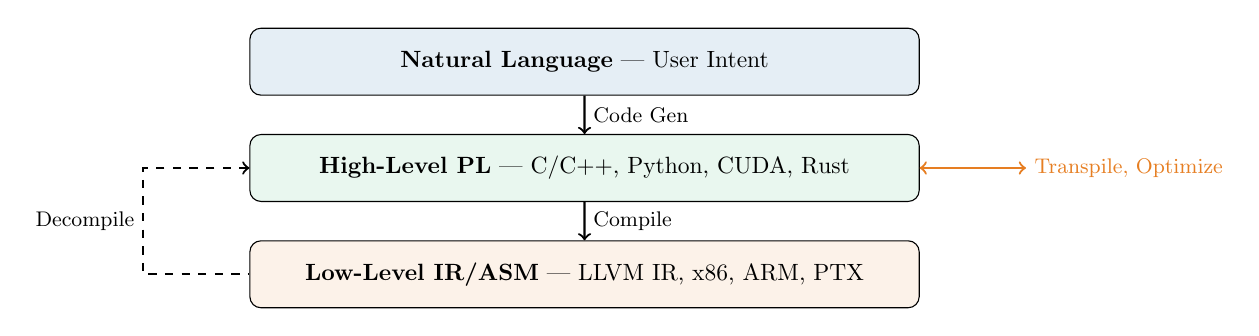
\begin{tikzpicture}[scale=0.9, every node/.style={scale=0.85}]
        % Levels
        \node[draw, rounded corners, minimum width=10cm, minimum height=1cm, fill=primaryblue!10] (nl) at (0,3) {\textbf{Natural Language} — User Intent};
        \node[draw, rounded corners, minimum width=10cm, minimum height=1cm, fill=successgreen!10] (pl) at (0,1.5) {\textbf{High-Level PL} — C/C++, Python, CUDA, Rust};
        \node[draw, rounded corners, minimum width=10cm, minimum height=1cm, fill=accentorange!10] (ir) at (0,0) {\textbf{Low-Level IR/ASM} — LLVM IR, x86, ARM, PTX};
        
        % Arrows
        \draw[->, thick] (nl) -- node[right]{\small Code Gen} (pl);
        \draw[->, thick] (pl) -- node[right]{\small Compile} (ir);
        \draw[<-, thick, dashed] (pl.west) -- ++(-1.5,0) |- node[pos=0.25, left]{\small Decompile} (ir.west);
        
        % Intra-level
        \draw[<->, thick, accentorange] (pl.east) -- ++(1.5,0) node[right]{\small Transpile, Optimize};
    \end{tikzpicture}
    \end{center}
    
    \textbf{Key Tasks:}
    \begin{itemize}
        \item \textbf{Transpilation}: C→Rust, CUDA→HIP, Java→Python
        \item \textbf{Code Optimization}: Performance tuning, parallelization
        \item \textbf{IR Optimization}: LLVM pass selection, code size reduction
        \item \textbf{Automated Repair}: Bug fixing as translation (buggy→correct)
    \end{itemize}
\end{frame}

\begin{frame}{Compiler.next: Intent → Optimized FMware}
    \begin{block}{Core Idea}
    Treat \textbf{human intent} as source code, compile it into optimized \textbf{FMware} (prompts + RAG + configs).
    \end{block}
    
    \begin{center}
    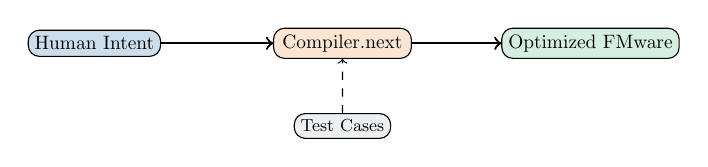
\begin{tikzpicture}[scale=0.7, every node/.style={scale=0.7}]
        \node[draw, rounded corners, fill=primaryblue!20, minimum width=2.2cm] (intent) at (0,0) {Human Intent};
        \node[draw, rounded corners, fill=accentorange!20, minimum width=2.5cm] (compiler) at (4.5,0) {Compiler.next};
        \node[draw, rounded corners, fill=successgreen!20, minimum width=2.2cm] (fmware) at (9,0) {Optimized FMware};
        
        \draw[->, thick] (intent) -- (compiler);
        \draw[->, thick] (compiler) -- (fmware);
        
        \node[draw, rounded corners, fill=lightgray, minimum width=1.5cm, font=\small] (gold) at (4.5,-1.5) {Test Cases};
        \draw[->, dashed] (gold) -- (compiler);
    \end{tikzpicture}
    \end{center}
    
    \begin{columns}[T]
    \column{0.5\textwidth}
    \textbf{Key Mechanisms:}
    \begin{itemize}
        \item Search-based optimization (NSGA-II)
        \item Multi-objective: accuracy vs cost vs latency
        \item Self-reflection \& semantic caching
    \end{itemize}
    
    \column{0.5\textwidth}
    \textbf{Results (HumanEval-Plus):}
    \begin{itemize}
        \item Accuracy: \textcolor{successgreen}{+47\%}
        \item Latency: \textcolor{successgreen}{-42\%}
        \item Token usage: \textcolor{successgreen}{-16\%}
    \end{itemize}
    \end{columns}
\end{frame}

%=============================================================================
\section{Key Challenges}
%=============================================================================

\begin{frame}{Challenge 1: Correctness \& Verification}
    \begin{alertblock}{The Fundamental Problem}
    LLMs are \textbf{probabilistic} — they can ``hallucinate'' incorrect code.
    \end{alertblock}
    
    \textbf{Manifestations:}
    \begin{itemize}
        \item Syntactically correct but semantically wrong
        \item Works on test cases but fails in production
        \item Subtle bugs in edge cases
    \end{itemize}
    
    \textbf{Current Approaches:}
    \begin{itemize}
        \item Unit test validation
        \item SMT solvers (e.g., alive2 for LLVM)
        \item Iterative repair with compiler feedback
        \item Symbolic execution
    \end{itemize}
    
    \textbf{Open Question:} How to verify correctness at scale without exhaustive testing?
\end{frame}

\begin{frame}{Challenge 2: Scalability \& Long Context}
    \begin{columns}[T]
    \column{0.5\textwidth}
    \textbf{Context Window Limits}
    \begin{itemize}
        \item Real codebases: millions of lines
        \item LLM context: 128K-1M tokens
        \item Cannot fit entire project
    \end{itemize}
    
    \textbf{Approaches:}
    \begin{itemize}
        \item Chunking \& retrieval (RAG)
        \item Hierarchical summarization
        \item Divide-and-conquer
    \end{itemize}
    
    \column{0.5\textwidth}
    \textbf{Project-Level Tasks}
    \begin{itemize}
        \item Cross-file dependencies
        \item Build system integration
        \item Long-horizon planning
    \end{itemize}
    
    \textbf{Current Limitations:}
    \begin{itemize}
        \item Lose global context
        \item Inconsistent across chunks
        \item Memory fragmentation
    \end{itemize}
    \end{columns}
\end{frame}

\begin{frame}{Challenge 3: Evaluation \& Benchmarks}
    \textbf{Current Benchmarks are Limited:}
    \begin{itemize}
        \item \textbf{HumanEval, MBPP}: Function-level, Python-only
        \item \textbf{SWE-Bench}: Project-level but limited interaction
        \item Most focus on code generation, not transformation/maintenance
    \end{itemize}
    
    \vspace{0.5em}
    \textbf{Missing Dimensions:}
    \begin{itemize}
        \item Multi-turn, interactive workflows
        \item Tool integration (compilers, debuggers)
        \item Real-world maintenance tasks
        \item Low-resource languages
        \item Long-horizon planning
    \end{itemize}
    
    \begin{alertblock}{Data Contamination}
    Many benchmarks are on GitHub → models may have seen solutions during training!
    \end{alertblock}
\end{frame}

\begin{frame}{Challenge 4: Tool Integration}
    \textbf{The Gap:}
    \begin{itemize}
        \item Programming tools designed for \textbf{humans}
        \item Error messages optimized for human readability
        \item Internal states hidden from automated systems
    \end{itemize}
    
    \textbf{What AI Agents Need:}
    \begin{itemize}
        \item Structured feedback (not just error strings)
        \item Access to intermediate representations
        \item Transformation traces
        \item Fine-grained state tracking
    \end{itemize}
    
    \begin{exampleblock}{Vision}
    Compilers \& languages should evolve to be \textbf{agent-aware} — exposing machine-consumable interfaces.
    \end{exampleblock}
\end{frame}

\begin{frame}{More Challenges}
    \begin{columns}[T]
    \column{0.5\textwidth}
    \textbf{Reproducibility}
    \begin{itemize}
        \item FM outputs are non-deterministic
        \item Same input → different outputs
        \item Hard to audit/verify
    \end{itemize}
    
    \vspace{0.5em}
    \textbf{Cost \& Efficiency}
    \begin{itemize}
        \item FM inference is expensive
        \item Search requires many evaluations
        \item Need caching, compression
    \end{itemize}
    
    \column{0.5\textwidth}
    \textbf{Human-AI Collaboration}
    \begin{itemize}
        \item When to defer to human?
        \item How to maintain trust?
        \item Explainability of decisions
    \end{itemize}
    
    \vspace{0.5em}
    \textbf{Low-Resource Domains}
    \begin{itemize}
        \item Rare languages (COBOL, OCaml)
        \item Specialized libraries
        \item Domain-specific knowledge
    \end{itemize}
    \end{columns}
\end{frame}

%=============================================================================
\section{Future Directions}
%=============================================================================

\begin{frame}{Research Directions}
    \begin{columns}[T]
    \column{0.5\textwidth}
    \textbf{AI for SE:}
    \begin{itemize}
        \item Automatic data curation
        \item RL for code optimization
        \item Better tool interfaces
        \item Human-AI collaboration
    \end{itemize}
    
    \column{0.5\textwidth}
    \textbf{New Compiler Stack:}
    \begin{itemize}
        \item Hybrid systems (LLM + traditional)
        \item Self-improving compilers
        \item Cross-level transformations
        \item Reproducible FM compilations
    \end{itemize}
    \end{columns}
    
    \vspace{1em}
    \begin{block}{Common Theme}
    Bridge the gap between LLM flexibility and traditional compiler reliability.
    \end{block}
\end{frame}

\begin{frame}{The Hybrid Future}
    \begin{center}
    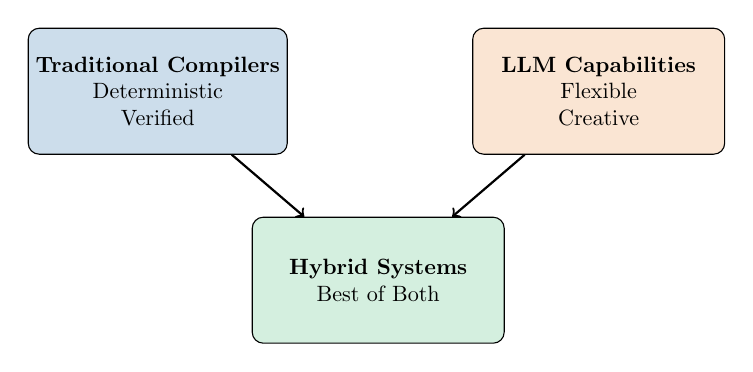
\begin{tikzpicture}[scale=0.8, every node/.style={scale=0.8, align=center}]
        \node[draw, rounded corners, fill=primaryblue!20, minimum width=4cm, minimum height=2cm] (traditional) at (0,0) {\textbf{Traditional Compilers}\\Deterministic\\Verified};
        
        \node[draw, rounded corners, fill=accentorange!20, minimum width=4cm, minimum height=2cm] (llm) at (7,0) {\textbf{LLM Capabilities}\\Flexible\\Creative};
        
        \node[draw, rounded corners, fill=successgreen!20, minimum width=4cm, minimum height=2cm] (hybrid) at (3.5,-3) {\textbf{Hybrid Systems}\\Best of Both};
        
        \draw[->, thick] (traditional) -- (hybrid);
        \draw[->, thick] (llm) -- (hybrid);
    \end{tikzpicture}
    \end{center}
    
    \textbf{Key Insight:} The most promising path combines:
    \begin{itemize}
        \item LLM creativity for exploration
        \item Traditional verification for correctness
        \item Human oversight for critical decisions
    \end{itemize}
\end{frame}

%=============================================================================
\section{Conclusion}
%=============================================================================

\begin{frame}{Key Takeaways}
    \begin{enumerate}
        \item \textbf{AI is transforming SE} — from code completion to autonomous agents
        
        \item \textbf{LLMs in Compilers} — selector/translator/generator patterns; intent → optimized FMware
        
        \item \textbf{Significant challenges remain}:
        \begin{itemize}
            \item Correctness \& verification
            \item Scalability to real projects
            \item Evaluation \& benchmarks
            \item Tool integration
        \end{itemize}
        
        \item \textbf{Hybrid systems} are the promising path forward
    \end{enumerate}
    
    \begin{block}{The Vision}
    Humans focus on \textit{what to build} and \textit{tradeoffs}; AI handles routine development.\strut
    \end{block}
\end{frame}

\begin{frame}{References}
    \small
    \begin{itemize}
        \item Gu et al., ``Challenges and Paths Towards AI for Software Engineering,'' 2025
        \item Wang et al., ``AI Agentic Programming: A Survey,'' 2025
        \item Zhang et al., ``The New Compiler Stack: A Survey on LLMs and Compilers,'' 2026
        \item Cogo et al., ``Compiler.next: A Search-Based Compiler for SE 3.0,'' 2025
    \end{itemize}
    
    \vspace{1em}
    \textbf{Key Benchmarks:}
    \begin{itemize}
        \item HumanEval, MBPP — Function-level code generation
        \item SWE-Bench — Project-level software engineering
        \item LiveCodeBench — Temporal evaluation
    \end{itemize}
\end{frame}

\begin{frame}[standout]
    Questions?
\end{frame}

\end{document}
